\documentclass[a4paper,12pt]{article}
%\usepackage[catalan]{babel}
\usepackage[utf8]{inputenc}
\usepackage{amsfonts}
\usepackage[colorlinks=true]{hyperref}
\usepackage[left=2.5cm,right=2.5cm]{geometry}
\usepackage{graphicx}
\usepackage[labelformat=empty]{caption}

\title{The Sphere of the Earth \\ Activities \\ {\small December 20, 2012  } }
\author{Daniel Ramos \footnote{E-mail: \texttt{daniel.ramos@mmaca.cat}}\\MMACA (Museu de Matemàtiques de Catalunya)}

\date{}

\pagestyle{empty}

\begin{document}
\maketitle \thispagestyle{empty}


These activities are designed to be done with the materials, posters and software of the exhibit ``The Sphere of the Earth''. This material
is given as a base reference, it can be elaborated on the form of a lecture, or can be printed on the walls next to the exhibits. This
material has not been exhaustively corrected. Some typos and mistakes may exist. Read carefully before using on a public exhibition and
report any issue to the author.

\vspace{4em}
A proposed use is as follows: Use section 1 as introductory material, close to a table with the globe and the tools. Display each section
2-7 on a panel next to its corresponding poster in a near wall. Display section 8 next to the computer, to be used after watching the
posters. Use section 9 as a complementary material for interested public.


%\thanks{Universitat Autònoma de Barcelona, Departament de Matemàtiques - 80193 Bellaterra, Barcelona (Spain)- \\ E-mail:
%\texttt{dramos@mat.uab.cat} . }


\newpage
\section{What is a map?}
A \emph{map projection} is a flat representation of the surface of the Earth. There are infinitely many ways of representing the Earth on a
plane, but all of them will distort its appearance in one way or another. Depending on the purpose of our map, we may need to preserve
faithfully some properties of the Earth at the expenses of losing others. For instance, on a navigational map it is important to keep track
of the angle between our route and the North, since we can compare it with the direction of the North on the compass. If we need to display
for instance climate regions of the Earth, it will be much more useful to use a map that does not distort areas.

\begin{itemize}
 \item Look at the Earth globe on the table and to these some relevant maps of the Earth. Do they all resemble the Earth? Can you feel or explain the distortion of each map?
 \item Look at the grid on the globe and on the maps. What is its use? Does it help on viewing the distortion?
\end{itemize}

\subsection*{Coordinates}
The system of coordinates on the Earth is a way of locating a point by means of two numbers: a \emph{longitude} ($\lambda$) and a \emph{latitude} ($\phi$). On the Earth, the fixed references are the North and South poles (the axis of the Earth), the equatorial plane (perpendicular to the axis), and the half-plane containing the Greenwich Royal Observatory and the axis of the Earth. Given a point on the Earth, its longitude is the angle between the half-plane containing $p$ and the axis of the Earth and the half-plane of Greenwich. The latitude is the angle between the line joining the center of the Earth with $p$ and the equatorial plane.
\begin{itemize}
 \item Identify longitude and latitude on the transparent model on the table.
\end{itemize}
Lines of equal longitude are called \emph{meridians}, and lines of equal latitude are called \emph{parallels}. Some of these lines can be drawn to create a grid called \emph{graticule}. The globe and the maps have a graticule spaced 10º on each coordinate.

Over the globe, the distance between two points can be measured as a length (in kilometers) or as the angle arc defined by the two points and the center of the Earth as the vertex (in degrees or radians). Recall that $arc\ length = angle  \cdot  radius$ (expressing the angle in radians).
\begin{itemize}
 \item Try to find the approximate coordinates of some cities on the globe and on the maps.
 \item Use the flexible ruler to measure some distances. Observe that there are two scales: on kilometers and on degrees.
\end{itemize}





\newpage
\section{The Plate-Carrée projection}
This is maybe the easiest projection. One just writes the longitude and latitude as the $x$ and $y$ coordinates of the plane. Therefore the
graticule forms an evenly distributed square grid. Is this representation faithful?
\begin{itemize}
 \item Each square on the graticule represents 10º on the Earth. But do the graticule on the Earth is ``squared''? Check a ``square'' of the graticule near the equator and near the poles on the globe. Do they have sides of equal length?. How much measures 10º of an arc of parallel at the equator? And at latitude 70ºN?
 \item Do the flexible ruler work on this map? 
\end{itemize}
To be more faithful, the graticule shouldn't be a square grid.




 
\newpage
\section{The Mercator projection}
This projection was invented by Gerardus Mercator in 1569, and is with no doubt the most important map projection in History. Most general
use maps are in this projection. Observe carefully a ``square'' on the graticule on the Earth globe, close to the poles. These ``squares''
are much more like rectangles. The Mercator projection is a vertical deformation of the Plate-Carrée projection. Since the parallels
appeared longer than they are, the meridians have been stretched the same amount, so that the map is equally stretched vertically and
horizontally at each point. The regions and areas are greatly distorted, but on the other hand we achieve an important feature: shapes and
angles are preserved.

A key feature for navigation is the following: Imagine you want to sail from a city to another across an ocean. You can draw the straight line joining these cities on the Mercator map. This line (called \emph{loxodrome} or rhumb line) makes a constant angle with the vertical meridians, pointing Northwards. Since the angles are preserved, this is the true angle you need to keep constant with your compass on your boat (although you should correct the small difference between magnetic and geographic North). Thus the Mercator map allows, and allowed during centuries, to find a path between two points on the globe. Beware: this loxodrome is only a path easy to follow, not the shortest!

\begin{itemize}
 \item Imagine you are in 16th century and you want to navigate from Cadiz (Southern Spain) to Caracas (today Venezuela) in your caravel.
Which is the easiest route (loxodrome) to follow? Use the plane protractor.

 \item Imagine you want to fly in present day from Athens (Greece) to Los Angeles (USA). Which is the loxodrome joining this two cities? 

If you actually take a plane covering a direct route from Athens to Los Angeles, you will find that you fly over a large snow land. It's
Greenland. Why? Check the shortest route on the globe.

 \item Use the spherical and plane protractors to check the equality of angles on the loxodrome in the map and in the globe.
\end{itemize}



\newpage
\section{The Gall-Peters projection}
Mercator projections tries to fix the deformation of the Plate-Carrée projection by correctiong the angles, but this distorts greatly
surfaces and areas. Other projections, such as Gall-Peters', can be designed to preserve areas. Gall-Peters map is said to be a ``third
world map'' because countries in Africa and South America (and all regions close to the equator) are given a preeminent place. If
Africa appears bigger than Europe is because it actually \emph{is} bigger (areas are correct). However, shape is not preserved. Africa is
not as skinny as it appears on this map.

\begin{itemize}
 \item Which continent is bigger, North America or Africa? Answer looking at the Gall-Peters projection. Would you say the same looking at
the Mercator projection? (Answer: North America is about $24,709,000\ \mathrm{km}^2$ an Africa about $30,221,532\ \mathrm{km}^2$.)

 \item Use the profiles in foam plastic sheets to compare the sizes of the continents on the map with the true spherical continents. Do
them fit? What happens with Antarctica?
\end{itemize}



\newpage
\section{The Azimuthal Equidistant projection}
This is the ``airport map''. Located at the center of the map is Barcelona (but you could choose any point on Earth). After fixing the
center, we draw points at equal distance to Barcelona over concentric circles around the center, using this distance as the radius. Thus,
the distance from Barcelona to any point of the Earth is displayed correctly over this map (but only distances from Barcelona!). The angle
between the radius joining Barcelona and the destination point and the North of the map (vertical direction) is also correct. Thus this is a
very useful map to have at Barcelona's airport, since you can get a good idea of how long is your journey and which countries are you flying
over. You can also see how far are different cities.

You can use the flexible ruler over this map, but only if you measure distances from Barcelona; otherwise your measure will be
wrong. 
\begin{itemize}
 \item How far are New York (USA), Cape Town (South Africa) and Tokio (Japan)?
 \item What is the diameter of this map?
 \item How many countries can you visit traveling less than 10,000 km?
 \item The antipodes of Barcelona (the point on Earth diametrically oposed to Barcelona) is a point on the Pacific Ocean, near New Zealand.
Where is this point on the map? Where is new Zealand?
\end{itemize}



\newpage
\section{The Gnomonic Projection}
This map seems highly distorted. However, it has a unique feature: all shortest paths on Earth (geodesics) are drawn as straight lines.
Thus, if you want that the shortest path between two points to be (to appear) the straight line, you must distort the map so much. Also,
not all the Earth can be displayed, only a small portion smaller than a half-sphere. The center of the projection is taken at Barcelona.
You can achieve this map projecting each point on Earth's surface from the center of the Earth onto a tangent plane at Barcelona.

\begin{itemize}
 \item Find the shortest path from Jerusalem (Israel) to La Habana (Cuba). Does it cross Africa? Would you say that looking at other
projections?
 \item What shape adopt parallels and meridians?
\end{itemize}





\newpage
\section{The Mollweide projection}
This projection fills an ellipse with axes in proportion 2:1. It solves partially a problem with all cylindrical projections (such as
Plate-Carrée, Mercator, Gall-Peters and others), namely that the poles are not displayed at one unique location. North pole on Plate-Carrée
corresponds to the whole upper border of the map rectangle. This distorts hugely regions around the poles, such as the Antarctica.
Mollweide projections solves this and reduces this distortion. Furthermore, Mollweide projection is equal-area, that is, the areas of
regions are preserved. Also, its rounded shape reminds the sphericity of the Earth, which is not aparent on other squared maps.

\begin{itemize}
 \item How are displayed parallels and meridians?
 \item Compare this projection with Gall-Peters projection. Both are equal-area. Which one do you think distort least the Earth? Use the
foam profiles of both projections and the globe.
\end{itemize}



\newpage
\section{Can we measure the distortion?}
The distortion of a map is a complicated magnitude that cannot be completelly measured by a single number. Instead, the French
mathematician Nicolas Auguste Tissot invented in 1859 a graphical method to display the distortion produced at any point on a map. Imagine
a small circle around a point on the Earth. If we project this circle onto the map, it will no longer appear as a circle, beacuse of the
distortion. If the circle is small enough (an infinitesimal circle), it will be projected onto an ellipse (an infinitesimal ellipse). We
can display this ellipse magnified so we can see it on the map. This ellipse is called a \emph{Tissot's indicatrix} for the map, and gives
several informations about the distortion.
\begin{figure}[h]
 \begin{center}
  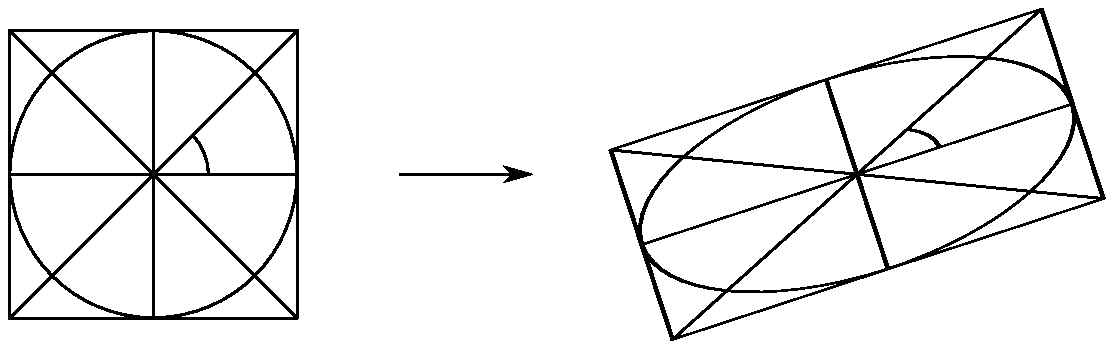
\includegraphics[width=0.7\textwidth]{tiss_diagram} 
\caption{An infinitesimal circle is projected onto an infinitesimal ellipse.}%\label{tiss_diagram}
 \end{center}
\end{figure}
\vspace{-1em}
\begin{itemize}
 \item Look at the program on the screen. You can select a map on the upper tabs. When you move the pointer over the map, the Tissot's
ellipse for that point appears over the map. Click over the map to leave the ellipse printed. You can choose the size of the ellipses and
clear all of them.
\end{itemize}



\paragraph{Principal directions.} We can think on the distortion as shrinking and stretching a map. However, we can shrink the map on one
direction and stretching on another direction, and this differently on every point on the map. The two axes of Tissot's
ellipse indicate the \emph{principal directions}, these are the directions on which the stretching is maximal and minimal. A very
flattened ellipse means that the distortion is very different in one or another direction. 
\begin{itemize}
 \item Which maps have more extreme ellipses? How do they look?
 \item How is the ellipse at the North pole on the Plate Carrée projection? Where is the North pole?
 \item Are the principal directions always the same as the meridian and parallel directions?
\end{itemize}



\paragraph{Conformality.} A Tissot's ellipse with equal axes (a circle) means that the distortion is equally big on any direction from that
point. Thus, any shape (such as the coast line) around this point is uniformly stretched on all direction, and hence the shape is
preserved. A map that preserves shape on every point is called \emph{conformal}. Observe in the diagram above that when the Tissot's ellipse
is a circle, all angles around the point are kept equal. \emph{Conformal maps preserve angles.}
\begin{itemize}
 \item When the Tissot's ellipse is a circle, the border of the ellipse turns green. Locate on each map the points where the map is
conformal.
 \item What's special on Mercator projection? How much are angles distorted? And areas?
\end{itemize}

\paragraph{Area.} The area of the ellipses tells us if the average distortion at this point is stretching or shrinking. If a small circle
of radius $r$ (with area $\pi r^2$) is projected onto an ellipse with semiaxis $a$ and $b$ (with area $\pi a b$) then, the condition $ab=r^2$
means that the area of the ellipse is the same as the circle, and therefore the map does not distort the area at this point (the amount of
shrinking on one direction compensates the stretching on another). A map that preserves area on every point is called \emph{equal-area}.

If a point on a map preserves shape and area (is conformal and equal-area) this point is said to be at \emph{true scale}. This point is
represented on the map without distortion. An important theorem in geometry says that there is no map with all poits at true scale, this
is, there is no perfect map.

\begin{itemize}
 \item When the area is preserved, the interior of the ellipse turns green. Which maps on the program are equal-area? What is the area of
the whole map on these cases?
 
 \item Let us compare the areas of Africa and Greenland. Use first Gall-Peters projection. Pick a medium or small size for the ellipses.
How many of them can you put over Greenland? and over Africa? Now repeat on the Mercator projection. Recall: Tissot's ellipses may seem
different, put \emph{represent the same disc over the Earth}. 

  The smaller the disc you pick, the better the approximation gets. The fact is that Africa is 14.2 times bigger than Greenland. Which
two maps reflect this proportion?

 \item Which is bigger: Greenland or Australia? Can you tell it looking only at the Plate Carrée Projection? And looking and using Tissot's
ellipses?

 \item Both Gall-Peters and Mollweide are equal-area maps. Which of them distorts less the shape? 


\end{itemize}



%\begin{figure}[!h]
 \begin{center}
  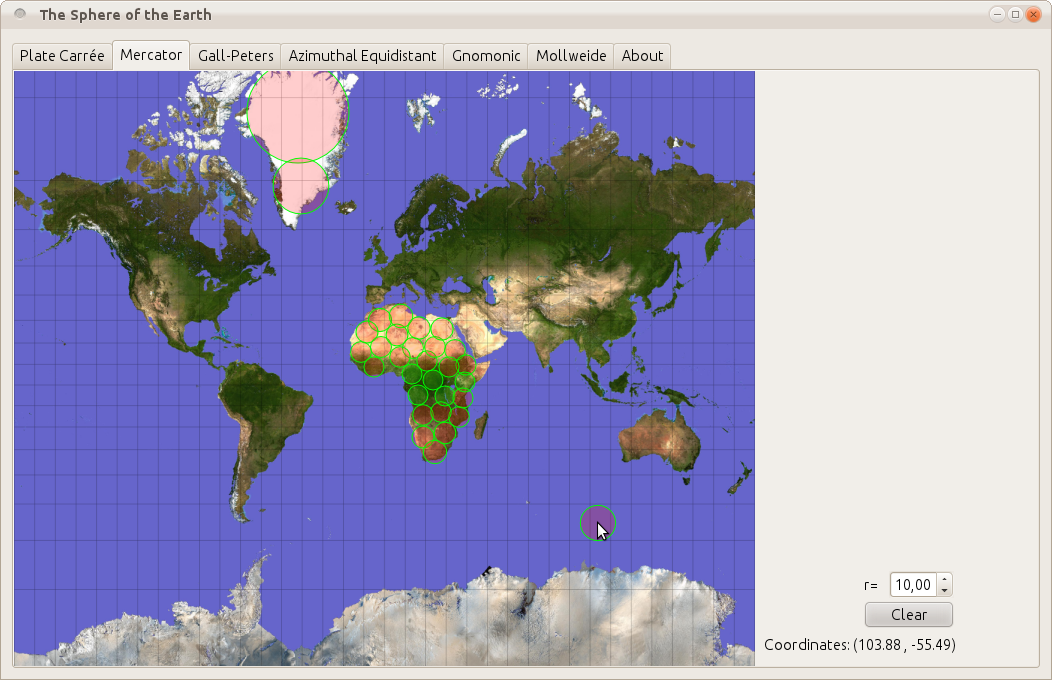
\includegraphics[width=0.7\textwidth]{merc1.png} 
  
{Comparison between the area of Africa and Greenland on the Mercator projection.}
 \end{center}
%\end{figure}




\newpage
\section{Inside mathematics}
\textsf{This section uses higher mathematics. Read at your own risk!} \\

A map projection sends every pair of coordinates on the sphere $\mathbb S$ to a pair of coordinates on the plane $\mathbb
R^2$,
$$\begin{array}{rccc}
   F: &\mathbb S & \longrightarrow & \mathbb R^2 \\
  & (\lambda, \phi) & \mapsto & (x,y)
  \end{array}
$$
where $\lambda$ is the longitude and $\phi$ the latitude. This mapping can be approximated by the differential function $dF$
$$\begin{array}{rccc}
   dF_p: & T_p \mathbb S & \longrightarrow & \mathbb R^2 
  \end{array}
$$
which sends the tangent plane to the sphere at $p$ to the plane $\mathbb R^2$ centered at $F(p)$. The tangent plane can be thought as the space of the directions on the point $p$, and the unit circle on the tangent plane at $p$ represent the set of all unitary directions from $p$. The Tissot's ellipse is the image by $dF$ of the unit circle on $T_p\mathbb S$. Hence, the Tissot's ellipse is a representation of \emph{how the directions from $p$ are distorted}.

\begin{figure}[h]
 \begin{center}
  \def\svgwidth{ 0.85 \textwidth}
\input{df.pdf_tex}
\caption{The map $F$ and its differential $dF$.}
 \end{center}
\end{figure}

There are two directions perpendiculars on the Earth that are also perpendicular on the map. To see that, consider a straight line $rs$ on the tangent plane and passing through $p$, and a half-line $t$ with origin at $p$, perpendicular to $rs$. Consider its image $r's'$ and $t'$ on the map plane passing through $p'=F(p)$, that need not to be perpendicular. Suppose for instance that $r'p't'$ is acute and $t'p's'$ is obtuse. Now imagine that we take the right angle $rpt$ and we rotate it around $p$, we begin at $rpt$ and finish at $tps$. On the map side, we begin at the acute angle  $r'p't'$ and finish at the obtuse $t'p's'$, thus, at some middle point we had a right angle as image. 

\begin{figure}[ht]
 \begin{center}
  \def\svgwidth{ 0.85 \textwidth}
\input{diagonalize.pdf_tex}
\caption{The principal directions are perpendicular.}
 \end{center}
\end{figure}


These two directions are the principal directions, represented by two perpendicular unitary vectors. The image of these two vectors give the principal directions on the map, and the length of these images, $a$, $b$, give the semiaxes of the Tissot's ellipse. If $a=b$ the ellipse is a circle, all the directions are distorted the same amount and the map is conformal at this point. If $ab=1$, the ellipse has the same area as the unitary disc on the tangent plane. Using an infinitesimal disc, we get the infinitesimal area on the sphere, and thus the map is area-preserving at this point.

On a formal language, we say that the differential $dF$ can be diagonalized with respect to the metric of the sphere, the eigenvectors give the principal directions and the eigenvalues give the semiaxes of the Tissot's ellipse. The conformality condition is that $dF$ is a multiple of the identity matrix, and the equal-area condition is $det(dF)=1$. Hold both conditions at every point would imply that $F$ is an isometry, but that's impossible because of Gauss' Egregium theorem.

 
 
\end{document}

